\documentclass{article}

\usepackage{fullpage}
\usepackage{amsmath}
\usepackage{algorithmic}
\usepackage{framed}
\usepackage{graphicx}


\newcommand{\literal}[1]{\fbox{\texttt{#1}}}
\newcommand{\sor}{\;\big|\;}

\begin{document}

This document details the architecture of the program that processes inference queries in various uncertainty metrics.

\section{Non-recursive data vs recursive data}

An important distinction that exists with data is whether it is non-recursive or recursive. 

\begin{itemize}
\item \textbf{Non-recursive data}: Envisioning the data as a directed graph, non-recursive data takes the form of a directed tree. All edges flow from the single root towards the leafs. Non-recursive data structures are the core of the program's architecture. Note that non-recursive data instances can be nested in other instances of the same types, but an instance cannot contain a chain of references back to itself, nor can two chains of references converge.
\item \textbf{Recursive data}: Envisioning the data as a directed graph, recursive data takes the form of an arbitrary directed graph, and can have loops both directed and undirected. Recursive data structures are the next layer of the program's architecture. Note that recursive data structures can reference themselves in any manner.
\end{itemize}

\section{endless arrays}

To aid with the implementation of various algorithms, a set of global arrays are maintained at all times:

The arrays are persistent, are extended on an as needs basis, but are never deallocated, ensuring that the allocated memory persists for the next call to an algorithm. 

There are two types of array sets that are maintained: arrays of bytes (whose class has the suffix \texttt{i} = ``inline"), and arrays of pointers (whose class has the suffix \texttt{p} = ``pointer").

The arrays are arranged in the following manner:

\begin{itemize}
\item At the top level, the arrays are grouped into layers/pages. A counter that indexes the current layer that is ``in use" is maintained. When a function is called, the counter is moved to the next layer so that the layer utilized by the parent function call remains unchanged. A the end of the function call, the counter is moved back to its previous value so that the parent function call can continue without its layer having been changed.
\item Within each layer, there is an ``array of arrays". There is an array of arrays as opposed to a single array due to the fact that some algorithms utilize more than 1 array.
\item When bytes are used instead of pointers, data is written to and read from the array in blocks.
\end{itemize}



\section{Non-recursive data}

\subsection{simple data}

The class simple data is a \textbf{non-recursive} unified data type that can store any data that does not have a recursive structure. The class stores a type identifier describing the \textbf{type} of data that is being referenced, and an anonymous pointer to the data itself. 

The following fields are present (the \textbf{bold} text denotes the data type):
\begin{description}
\item[\textbf{type\_identifier} \texttt{the\_type\_id}] stores an identifier for the \textbf{type} of data that is being referenced.    
\item[\textbf{int} \texttt{the\_type\_size}] stores the size of the data block that is being referenced.
\item[\textbf{void*} \texttt{the\_element}] is an anonymous pointer that references the data. 
\end{description}

The various data structure \textbf{type}s that can be stored as \texttt{simple\_data} are:
\begin{description}
\item[\textbf{void}]: (\texttt{the\_type\_id} = \texttt{TI\_VOID}) A null data structure.
\item[An array of bytes]: (\texttt{the\_type\_id} = \texttt{TI\_MEM\_BLOCK}) A generic array of bytes of length \texttt{the\_type\_size}. 
\item[\textbf{bool}]: (\texttt{the\_type\_id} = \texttt{TI\_BOOL}) A boolean value.
\item[\textbf{uchar}]: (\texttt{the\_type\_id} = \texttt{TI\_UCHAR}) An unsigned byte.
\item[\textbf{uint16}]: (\texttt{the\_type\_id} = \texttt{TI\_UINT16}) An unsigned 16-bit integer.
\item[\textbf{int}]: (\texttt{the\_type\_id} = \texttt{TI\_INT}) A signed 32-bit integer.
\item[\textbf{double}]: (\texttt{the\_type\_id} = \texttt{TI\_DOUBLE}) A long floating point number.
\item[\textbf{doublex}]: (\texttt{the\_type\_id} = \texttt{TI\_DOUBLEX}) A long floating point number that can attain special values such as \(+\infty\), \(-\infty\), and NaN.
\item[\textbf{fuzzy}]: (\texttt{the\_type\_id} = \texttt{TI\_FUZZY}) A triangular fuzzy number.
\item[\textbf{string}]: (\texttt{the\_type\_id} = \texttt{TI\_STRING}) A string of characters.
\item[\textbf{box}]: (\texttt{the\_type\_id} = \texttt{TI\_BOX}) A container class that contains a single simple\_data structure.
\item[\textbf{data\_pair}]: (\texttt{the\_type\_id} = \texttt{TI\_PAIR}) A pair of simple\_data structures.
\item[\textbf{list}]: (\texttt{the\_type\_id} = \texttt{TI\_LIST}) A list of simple\_data structures.
\end{description}


\subsection{boxes}

The ``box" is a simple container class with a single field that stores a single simple\_data instance. 

\subsection{pairs}

Often, simple data is needed to be bundled into pairs or more complex data structures to allow for collections of data to be passed from variable to variable. These structures are referred to as \textbf{data pair}s and are \textbf{non-recursive}.

\subsection{lists}

Similar to endless arrays, a common \textbf{non-recursive} data structure that will be encountered are arrays of simple\_data that can dynamically extend themselves as more entries are required. These dynamically adjustable arrays are referred to as \textbf{list}s.

\subsection{simple data ordering}

Given any two simple data values \(d_1\) and \(d_2\), an ordering is established such that it is always the case that exactly one of the following is true: \(d_1 < d_2\); \(d_1 = d_2\); or \(d_1 > d_2\). Simple data types are lumped together in the ordering, and the ordering of the simple data types is the same as the order in which the types are listed above.



\section{Recursive data}

\subsection{nodes}

A node is a node in a directed graph that are used to implement \textbf{recursive} data structures. Complex data structures such as decision trees/diagrams are manifested via a directed graph that is comprised of nodes.

A node consists of:
\begin{itemize}
\item A simple data field.
\item An ordered list of pointers to the child nodes. The list is indexed starting from 0.
\end{itemize}

%Each node maintains a list of both parent and child nodes. A node without parents and is vulnerable to deletion unless its existence is ``locked". 

%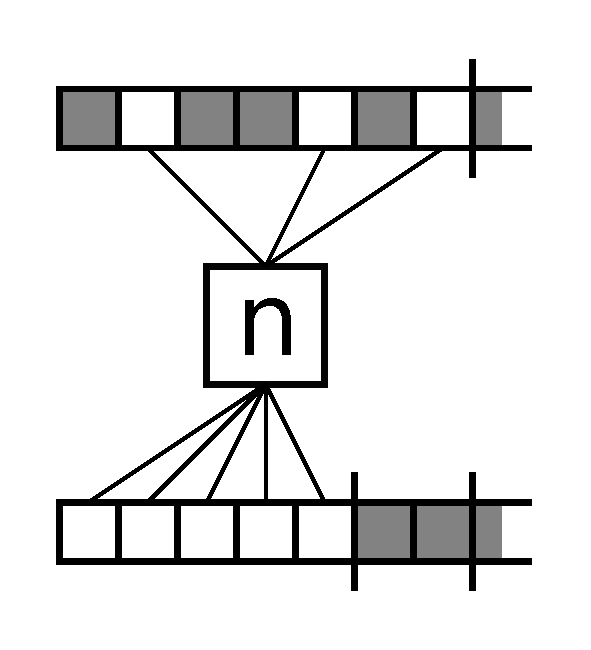
\includegraphics[width = 0.5\textwidth]{node_memory_structure}

%In addition to the child and parent lists, each node has a simple data field that holds the actual data that is assigned to the node. 



\subsection{sub-graph tracing}

Many subroutines that process a directed graph require that the subgraph that is rooted at the input node be traced in a depth-first fashion.

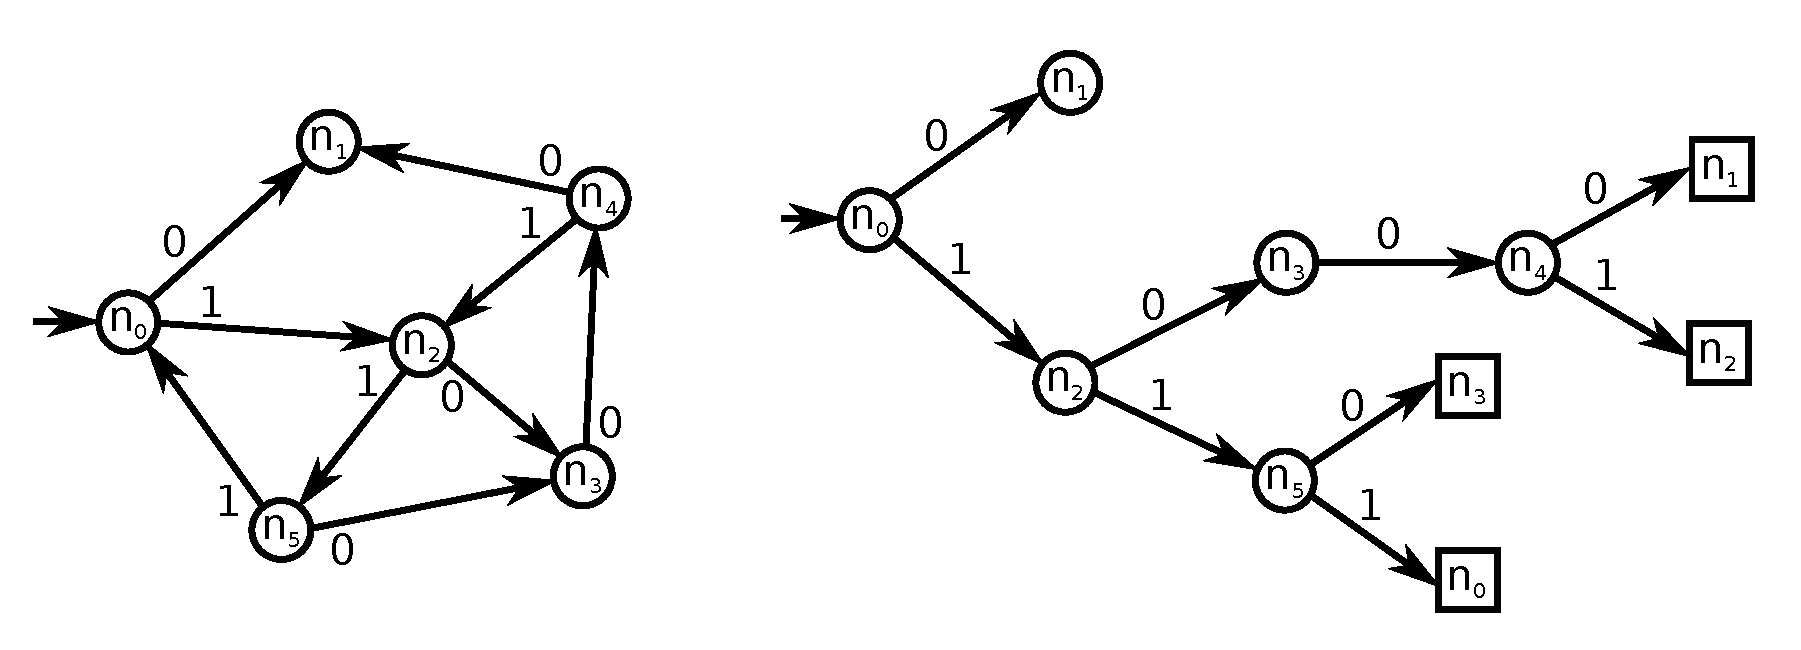
\includegraphics[width = \textwidth]{subgraph_with_tracer_tree}

The tracing in this example proceeds as follows: 

\begin{itemize}
\item Start at the root node \(n_0\).
\item Transition to child 0 of node \(n_0\), which is \(n_1\). 
\item Node \(n_1\) has no children, so backtrack to node \(n_0\). 
\item Transition to child 1 of \(n_0\) which is \(n_2\).
\item Transition to child 0 of \(n_2\) which is \(n_3\). 
\item Transition to child 0 of \(n_3\) which is \(n_4\).
\item Child 0 of \(n_4\) (which is \(n_1\)) has already been visited, so remain at \(n_4\).
\item Child 1 of \(n_4\) (which is \(n_2\)) has already been visited, so remain at \(n_4\). 
\item The children of \(n_4\) have been accounted for, so backtrack to \(n_3\).
\item The children of \(n_3\) have been accounted for, so backtrack to \(n_2\). 
\item Transition to child 1 of \(n_2\) which is \(n_5\). 
\item Child 0 of \(n_5\) (which is \(n_3\)) has already been visited, so remain at \(n_5\).
\item Child 1 of \(n_5\) (which is \(n_0\)) has already been visited, so remain at \(n_5\). 
\item The children of \(n_5\) have been accounted for, so backtrack to \(n_2\). 
\item The children of \(n_2\) have been accounted for, so backtrack to \(n_0\).
\item The children of \(n_0\) have been accounted for, so the trace finishes.
\end{itemize}


\subsection{product subgraphs}

\begin{tabular}{cc}
\fbox{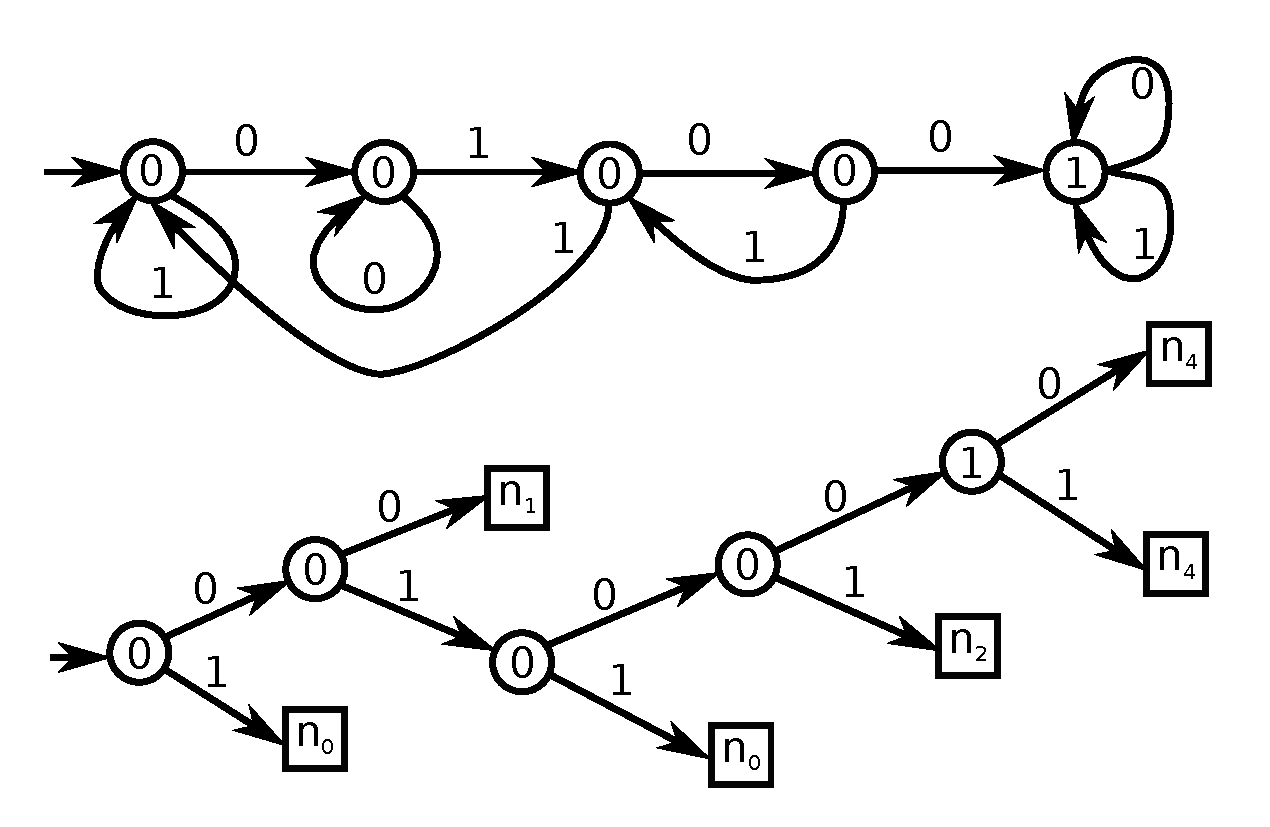
\includegraphics[width = 0.45\textwidth]{finite_automa_1}} & 
\fbox{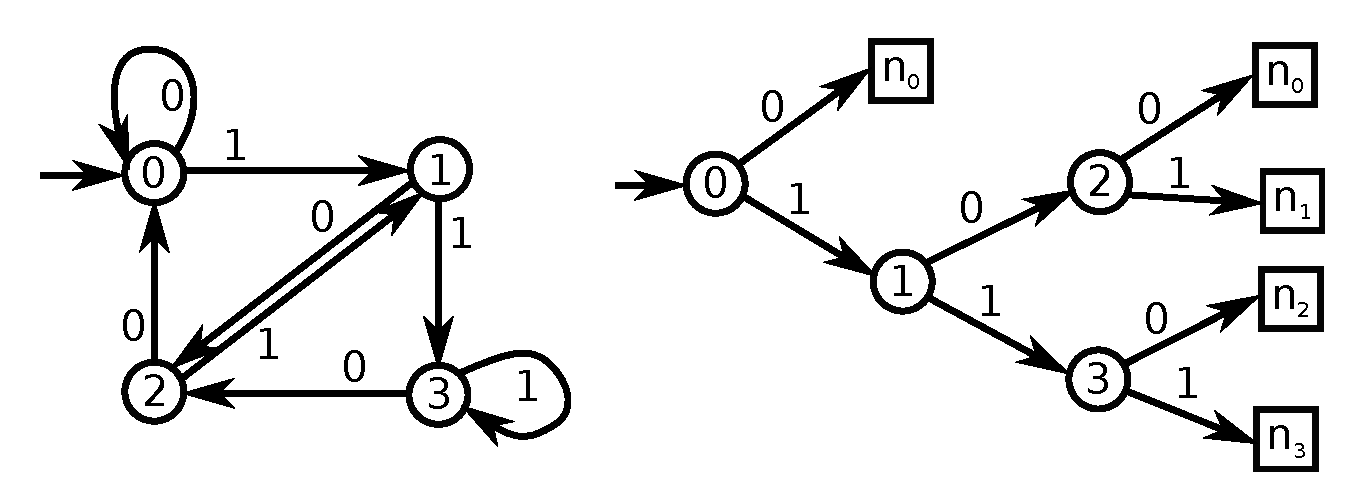
\includegraphics[width = 0.45\textwidth]{finite_automa_2}} \\ 
\fbox{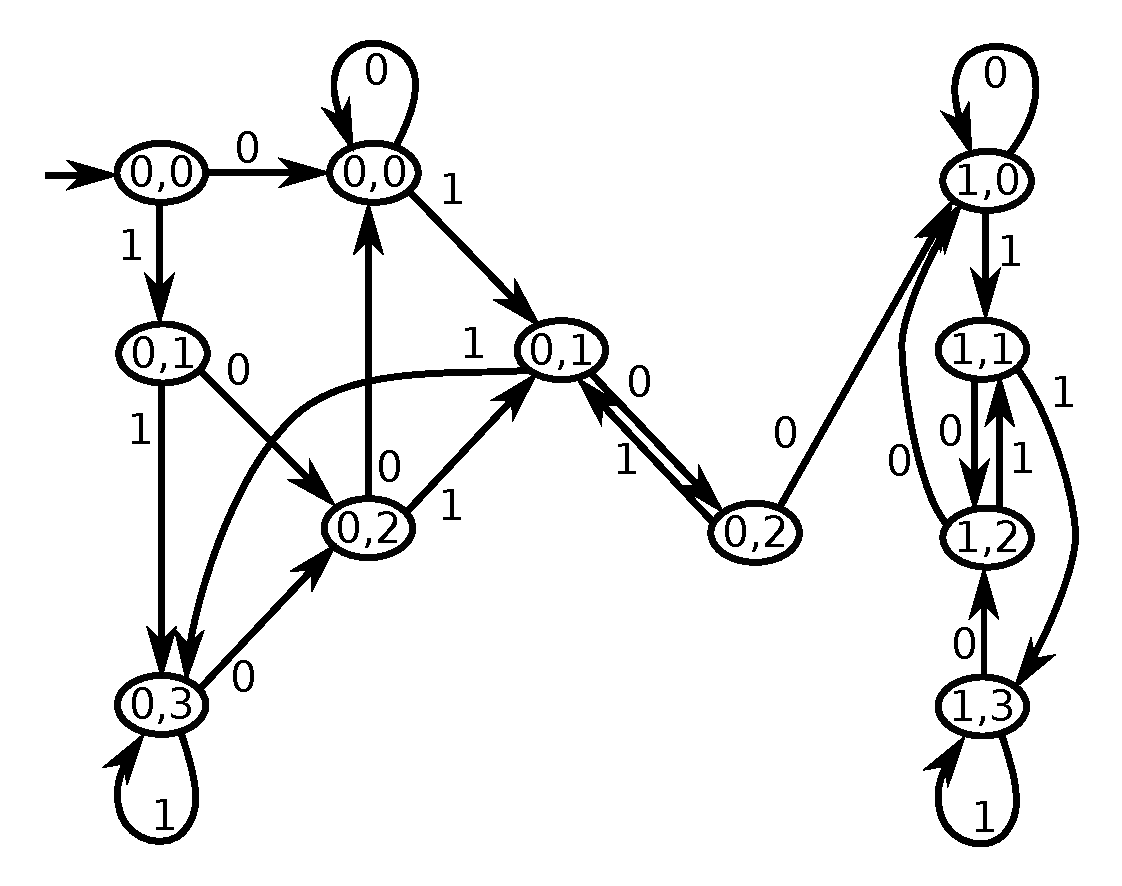
\includegraphics[width = 0.45\textwidth]{finite_automa_1x2}} &  
\end{tabular}

\vspace{5mm}

Top left: A directed graph and its associated depth-first tracer tree that denotes a finite state machine that returns 1 if and only if the sequence 0100 is detected.

Top right: A directed graph and its associated depth-first tracer tree that denotes a finite state machine that returns the decimal number equivalent to the final two bits of the input sequence.

Bottom left: The product directed graph of the two previous directed graphs. 



% ******************************* File Format *****************************

\section{File parsing and tokens}

\subsection{tokens}

All input files are parsed into tokens. The rules for extracting the tokens are described in detail below:

To aid in the description, the set of all characters is given the following taxonomy:

\begin{description}
\item[Alphabetic] ~
	\begin{description} 
	\item[All letters] \texttt{aAbB...zZ}
	\item[Underscore] \texttt{\_}
	\end{description}
\item[Numeric] \texttt{0123456789}
\item[Symbols] ~
	\begin{description}
	\item[sign] \texttt{+-}
	\item[decimal point] \texttt{.}
	\item[double quote] \texttt{"}
	\item[escape character] \texttt{\textbackslash}
	\item[other characters]
	\end{description}
\item[Whitespace] 
\end{description}

\vspace{5mm}

To aid in describing the tokens themselves, notation related to regular expressions will be used:
\begin{itemize}
\item \(\emptyset\) denotes the empty string.
\item \(\literal{literal}\) denotes the single string ``\(\text{literal}\)". 
\item \(\text{string}_1\text{string}_2\) denotes the concatenation of \(\text{string}_1\) and \(\text{string}_2\).
\item \((\text{option}_1\sor\text{option}_2\sor...\sor\text{option}_n)\) denotes a choice between options \(\text{option}_1\), \(\text{option}_2\), ..., \(\text{option}_n\).
\item \((\text{fragment})^*\) denotes ``\(\text{fragment}\)" repeated 0 or more times. The parentheses may be omitted if not necessary.
\item \((\text{fragment})^+\) denotes ``\(\text{fragment}\)" repeated 1 or more times. The parentheses may be omitted if not necessary.
\item \((\text{options}_2-\text{options}_1)\) denotes \(\text{options}_2\) with all options from ``\(\text{options}_1\)" excluded.
\item \(\mathbf{A}\) denotes an alphabetic character (including the underscore).
\item \(\mathbf{N}\) denotes an arbitrary numeric digit.
\item \(\mathbf{S}\) denotes an arbitrary symbol. 
\end{itemize}

The tokens themselves belong to one of the following categories:
\begin{description}
\item[Alpha-numeric] An alpha-numeric token starts with an alphabetic character (letters + underscore) and consists of any sequence of alphabetic and numeric characters. An alpha-numeric token ends on the last alphabetic or numeric character before a non alphabetic and non numeric character. The general form is 
\[\mathbf{A}(\mathbf{A}\sor\mathbf{N})^*\]
%*******************
\item[Integer] An integer token is continuous string of numeric characters where the first character may be \texttt{+} or \texttt{-}. At least one numeric character is required. The plus sign \texttt{+} or minus sign \texttt{-} on its own is a symbol. The general form is 
\[(\emptyset\sor\literal{+}\sor\literal{-})\mathbf{N}^+\]
%*******************
\item[Fixed-point] A fixed point number. The general form that is read is 
\[(\emptyset\sor\literal{+}\sor\literal{-})\mathbf{N}^*\literal{.}\mathbf{N}^*\] 
After processing, 0s pad the decimal point if necessary giving 
\[(\emptyset\sor\literal{+}\sor\literal{-})(\mathbf{N}^+\sor\literal{0})\literal{.}(\mathbf{N}^+\sor\literal{0})\]
%*******************
\item[Floating-point] A floating point number. The general form that is read is 
\[(\emptyset\sor\literal{+}\sor\literal{-})\mathbf{N}^*\literal{.}\mathbf{N}^*\literal{e}(\emptyset\sor\literal{+}\sor\literal{-})\mathbf{N}^*\] 
After processing, 0s pad the decimal point and exponent if necessary giving 
\[(\emptyset\sor\literal{+}\sor\literal{-})(\mathbf{N}^+\sor\literal{0})\literal{.}(\mathbf{N}^+\sor\literal{0})\literal{e}(\emptyset\sor\literal{+}\sor\literal{-})(\mathbf{N}^+\sor\literal{0})\]
%*******************
\item[String] A string of characters. The general form that is read is 
\[\literal{"}(((\mathbf{A}\sor\mathbf{N}\sor\mathbf{S})-(\literal{"}\sor\literal{\textbackslash}\sor\literal{\{}\sor\literal{\}}))\sor(\literal{\textbackslash}(\mathbf{A}\sor\mathbf{N}\sor\mathbf{S})))^*\literal{"}\]
After the encapsulating double quotes have been removed and the escape characters have been resolved, the general form is 
\[(\mathbf{A}\sor\mathbf{N}\sor\mathbf{S})^*\]
%*******************
\item[Symbol] An isolated symbol: 
\[\mathbf{S} - (\literal{.}\sor\literal{"}\sor\literal{\{}\sor\literal{\}})\]
\end{description}

\textbf{In addition, a comment is inert text that is skipped by the token reader. A comment is enclosed by curly braces \texttt{\{\}}.} 


%************************ SIMPLE DATA SYNTAX **********************
\subsection{simple data syntax}

For data input and output, it is necessary to represent simple data as a list of tokens that can be read or written by both a human and machine. This section will describe the text syntax that is used for various types using the same syntax for regular expressions that was described above. When whitespace is present, the amount of type of whitespace is irrelevant. The underlined text denotes fields that filled with relevant data. 
\begin{description}
\item[\textbf{void}]: \(\literal{0}\)
\item[An array of bytes]: No text representation. 
\item[\textbf{bool}]: \(\literal{bool }(\literal{0}\sor\literal{1})\)
\item[\textbf{uchar}]: \(\literal{c }\;\underline{\text{the character}}\)
\item[\textbf{uint16}]: \(\literal{uint16 }\;\underline{\text{the integer}}\)
\item[\textbf{int}]: \(\literal{i }\;\underline{\text{the integer}}\)
\item[\textbf{double}]: \(\literal{d }\;\underline{\text{the double}}\)
\item[\textbf{doublex}]: \(\literal{dx }\;(\underline{\text{the double}}\sor\literal{pos\_inf}\sor\literal{neg\_inf} \sor \literal{NaN})\)
\item[\textbf{fuzzy}]: \(\literal{fuzzy ( }\;\underline{\text{lower doublex}}\;\literal{ , }\;\underline{\text{center doublex}}\;\literal{ , }\;\underline{\text{upper doublex}}\;\literal{ )}\)
\item[\textbf{string}]: \(\literal{s "}\;\underline{\text{the string}}\;\literal{"}\) \\ 
Use \texttt{\textbackslash} to escape \texttt{\textbackslash}, \texttt{"}, \texttt{\{}, or \texttt{\}} (\texttt{\textbackslash\textbackslash} \(\mapsto\) \texttt{\textbackslash}; \texttt{\textbackslash"} \(\mapsto\) \texttt{"}; \texttt{\textbackslash\{} \(\mapsto\) \texttt{\{}; and \texttt{\textbackslash\}} \(\mapsto\) \texttt{\}})
\item[\textbf{box}]: \(\literal{box }\;\underline{\text{the data}}\)
\item[\textbf{data\_pair}]: \(\literal{pair < }\;\underline{\text{data 1}}\;\literal{ , }\;\underline{\text{data 2}}\;\literal{ >}\) 
\item[\textbf{list}]: \(\literal{list }\;\underline{\text{length}}\;\literal{ < }\;(\emptyset \sor (\underline{\text{data}}(\literal{ , }\;\underline{\text{data}})^*))\;\literal{ >}\) 
\end{description}


%************************ RECURSIVE DATA SYNTAX **********************
\subsection{recursive data syntax}

A directed graph starts with a definition of its root node.

A root node has the following syntax: 

\[\underline{\text{root node}} = (\underline{\text{new node}} \sor \underline{\text{molded table}})\]

\vspace{5mm}

An interior/child node has the following syntax: 

\[\underline{\text{child node}} = (\underline{\text{new node}} \sor \underline{\text{back reference}} \sor \underline{\text{molded table}})\]

The meaning of the fields \underline{\text{new node}}, \underline{\text{back reference}}, and \underline{\text{molded table}} are explained below:

\vspace{5mm}

%************************ NEW NODE SYNTAX **********************
\subsubsection{new node syntax}

A new node in the subgraph, denoted by field \underline{\text{new node}}, in the directed graph is represented in text via the following format:

\[\underline{\text{new node}} = \literal{new }\;\underline{\text{the data}}(\literal{ * } \sor (\literal{ < }\;\underline{\text{child node}}(\literal{ , }\;\underline{\text{child node}})^*\literal{ > }))\]

Field \underline{\text{the data}} refers to the data stored directly in the current node. 

The symbol \texttt{*} indicates the absence of children. A pair of triangular braces \texttt{< >} denotes a list of children separated by commas (\texttt{,}). 

%************************ BACK REFERENCES **********************
\subsubsection{back reference syntax}

A ``back reference", denoted by field \underline{\text{back reference}}, references a previously defined node in the subgraph's definition. 

\begin{description}
\item[absolute reference] Denoted by \(\literal{ref }\;\underline{\text{node index}}\), an absolute reference is an integer that indexes the referenced node's position (starting from 0) when the nodes are ordered according to when they were defined. 
\item[relative reference] Denoted by \(\literal{addr }\;\underline{\text{relative address}}\;\literal{ @}\), a relative reference is a list of symbols that describes the position of the referenced node relative to the node whose child is currently being described. The \underline{\text{relative address}} is a list of the following symbols. Starting with a reference to the node whose child is currently being described, 
\begin{itemize}
\item \texttt{!} moves the reference pointer to the root node. 
\item \texttt{\^} moves the reference pointer up to the prime parent of the node currently being referenced. The ``prime parent" of a node is the parent that precedes the node during a depth-first trace.
\item an integer token moves the reference pointer to the child indexed by the integer. 
\end{itemize}
\end{description}

%************************ MOLDED TABLES **********************
\subsubsection{molded table syntax}

In many scenarios, such as the representation of conditional probability tables, the directed graph depicts a multi-dimensional array in the form of a decision diagram. This decision diagram will often have a full tree structure except for some layers where the decision variables have no impact. In inactive decision layers, all children of each decision node reference the same child. Denoting a full tree using the above notation is often cumbersome, and a simpler approach would be to list all of the leaf values, alongside data describing the shape of the decision tree/diagram. 

A molded table, denoted by field \underline{\text{molded table}}, has the syntax:
\begin{align*}
& \underline{\text{molded table}} \\
& \;=\;\literal{table }\;\underline{\text{num of layers}}\;\literal{~}\;(\;\underline{\text{variable description}}\;\literal{~}\;)^*\;\literal{~}\;\underline{\text{default value}}\;\literal{~}\;(\underline{\text{array entry}}\;\literal{~})^+
\end{align*}

The field \underline{\text{variable description}} has the syntax: 
\begin{align*}
& \underline{\text{variable description}} \\
& \;=\; (\literal{normal }\sor\literal{inactive }\sor\literal{specific })\;\underline{\text{variable name}}\;\literal{~}\;\underline{\text{domain size}}\;\literal{~}\;(\emptyset\sor\underline{\text{specific child index}})
\end{align*}

Field \underline{\text{num of layers}} denotes the nonnegative number of decision layers in the decision tree, not counting the leaf node layer. The \underline{\text{num of layers}} field is followed by a list of details about each layer, starting from the root layer. Each description is denoted by the field \underline{\text{variable description}}, whose syntax is given above.

Each decision layer corresponds to a variable whose name is any simple data value. The variable's name, denoted by the field \underline{\text{variable name}} is assigned to the data field of each node in the variable's decision layer. In addition, all nodes in a variable's decision layer have the same number of children equal to the size of the variable's domain, indicated by the field \underline{\text{domain size}}. Each variable is one of three types described below: 
\begin{itemize}
\item \literal{normal } indicates that the children of each node in the current layer all reference different children, and that the variable has an impact on the decision. The field \underline{\text{specific child index}} is not used in this case.
\item \literal{inactive } indicates that the children of each node in the current layer all reference the same child. This effectively renders the variable ``inactive" in the decision making process. The field \underline{\text{specific child index}} is not used in this case.
\item \literal{specific } indicates that all child references except for the child indexed by \underline{\text{specific child index}} reference a node that leads to a leaf node labeled with the simple data \underline{\text{default value}}.
\end{itemize}

After the list of \underline{\text{variable description}} fields, a simple data default value \underline{\text{default value}} is provided, which is then followed by a list of simple data values \underline{\text{array entry}} that populate the data field of each leaf node.

%Molded table example 1
Below is shown an example molded table: the syntax on the left, and the manifested directed graph/decision diagram is shown on the right. There are 3 decision variables named \texttt{x0}, \texttt{x1}, and \texttt{x2}, with respective domain sizes 3, 2, and 2. Variables \texttt{x0} and \texttt{x2} are ``normal", while variable \texttt{x1} is ``inactive".

\begin{tabular}{cc}
\begin{minipage}[b]{0.4\textwidth}
\begin{verbatim}
table 3 
normal   s "x0" 3 
inactive s "x1" 2 
normal   s "x2" 2 
0 
d 0.4  d 0.7  d 0.2  d 0.1  d 0.9  d 0.8 
\end{verbatim}
\end{minipage} & 
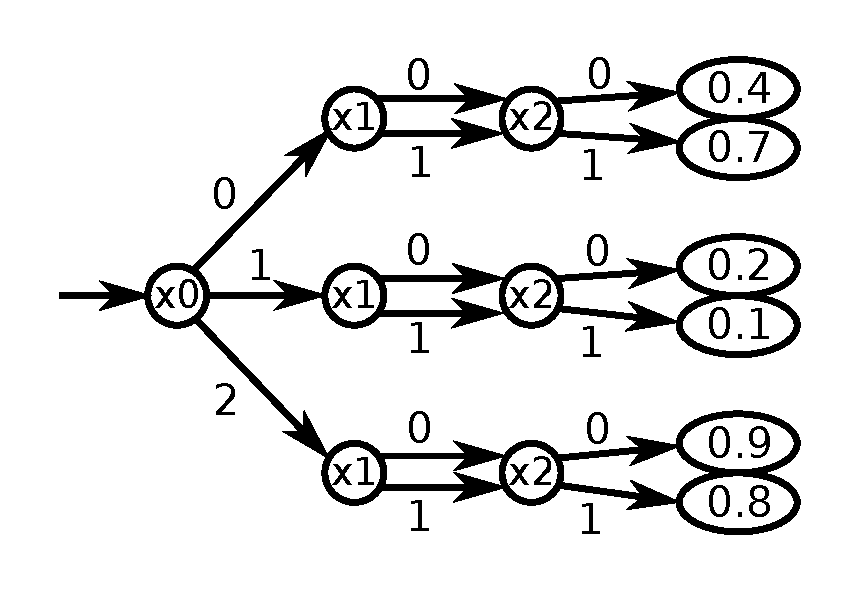
\includegraphics[width = 0.4\textwidth]{example_molded_array.pdf} \\
\end{tabular}

\vspace{5mm}

Without the molded table syntax, the decision diagram would be denoted by the following syntax:

\begin{verbatim}
new s "x0" < 
    new s "x1" < new s "x2" < 
        new d 0.4 * , 
        new d 0.7 * > , 
    addr 0 @ > , 
    new s "x1" < new s "x2" < 
        new d 0.2 * , 
        new d 0.1 * > , 
    addr 0 @ > , 
    new s "x1" < new s "x2" < 
        new d 0.9 * , 
        new d 0.8 * > , 
    addr 0 @ > >
\end{verbatim}

\vspace{5mm}

%Molded table example 2
Below is shown another example molded table: the syntax on the left, and the manifested directed graph/decision diagram is shown on the right. There are 3 decision variables named \texttt{x0}, \texttt{x1}, and \texttt{x2}, with respective domain sizes 3, 2, and 2. Variables \texttt{x0} and \texttt{x2} are ``normal", while variable \texttt{x1} is ``specific". For the nodes labeled with \texttt{x1}, all children except for child 1 reference an identity decision diagram that always returns the specified default value: \texttt{bool 1}

\begin{tabular}{cc}
\begin{minipage}[b]{0.4\textwidth}
\begin{verbatim}
table 3 
normal   s "x0" 3 
specific s "x1" 2 1
normal   s "x2" 2 
bool 1 
d 0.4  d 0.7  d 0.2  d 0.1  d 0.9  d 0.8 
\end{verbatim}
\end{minipage} & 
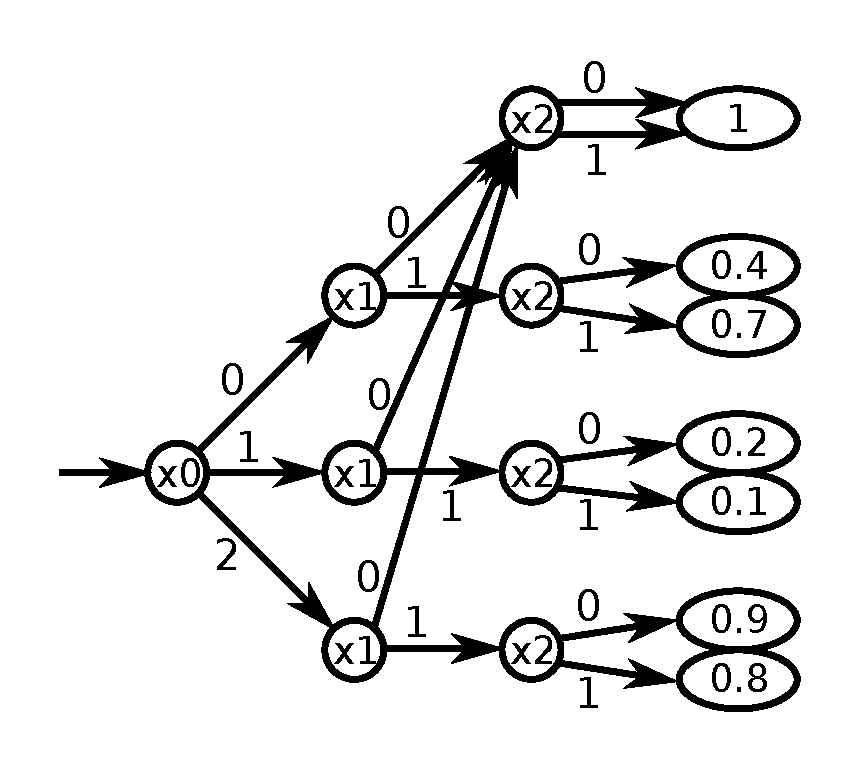
\includegraphics[width = 0.4\textwidth]{example_molded_array_2.pdf} \\
\end{tabular}

\vspace{5mm}

Without the molded table syntax, the decision diagram would be denoted by the following syntax:

\begin{verbatim}
new s "x0" < 
    new s "x1" < 
        new s "x2" < 
            new bool 1 * , 
            addr 0 @ > , 
        new s "x2" < 
            new d 0.4 * , 
            new d 0.7 * > > , 
    new s "x1" < 
        addr ! 0 0 @ , 
        new s "x2" < 
            new d 0.2 * , 
            new d 0.1 * > > , 
    new s "x1" < 
        addr ! 0 0 @ , 
        new s "x2" < 
            new d 0.9 * , 
            new d 0.8 * > > >  
\end{verbatim}

\vspace{5mm}


\subsubsection{example directed graph}

The following directed graph can be denoted by the following strings:

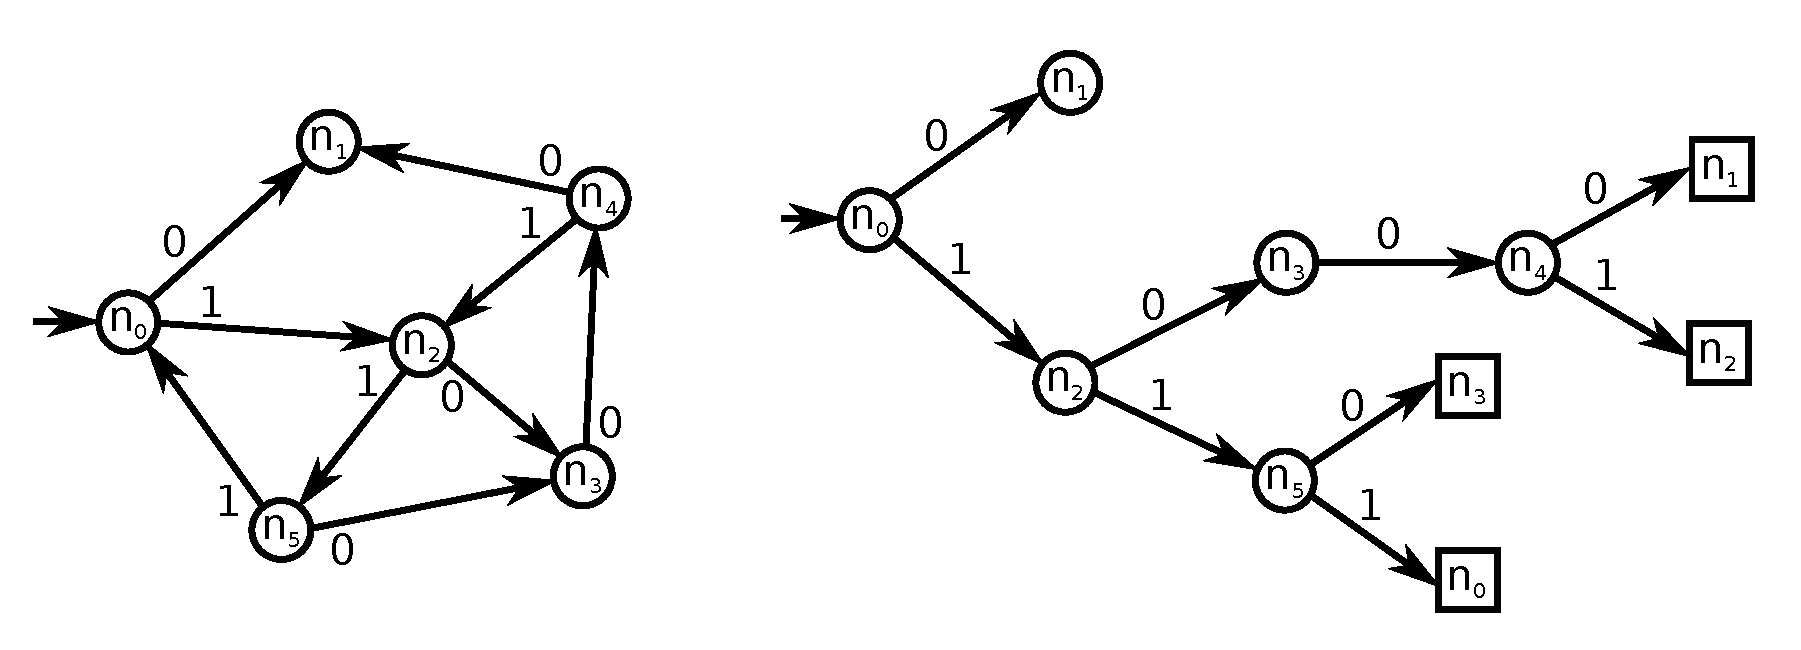
\includegraphics[width = \textwidth]{subgraph_with_tracer_tree}

The directed graph is shown on the left, while the depth-first tracer tree is shown on the right.

Using absolute back references gives the string:

\texttt{new s "n\_0" < new s "n\_1" * , new s "n\_2" < new s "n\_3" < new s "n\_4" < ref 1 , ref 2 > > , new s "n\_5" < ref 3 , ref 0 > > >}

Using relative back references gives the string: 

\texttt{new s "n\_0" < new s "n\_1" * , new s "n\_2" < new s "n\_3" < new s "n\_4" < addr !~0 @ , addr !~1 @ > > , new s "n\_5" < addr !~1 0 @ , addr !~@> > >}

or the string: 

\texttt{new s "n\_0" < new s "n\_1" * , new s "n\_2" < new s "n\_3" < new s "n\_4" < addr \^{} \^{} \^{} 0 @ , addr \^{} \^{} @ > > , new s "n\_5" < addr \^{} 0 @ , addr \^{} \^{} @ > > >}



\section{Arithmetic}

Arithmetic can be performed on elements of all data types, even on elements with different data types. The main unary operators are negation and inverting, and the main binary operators are addition and multiplication. 



\section{Input Syntax}

Given an experiment number \(i\), two input files are required: ``\texttt{Test Files/\(i\)\_data.txt}" and \\ ``\texttt{Test Files/\(i\)\_instructions.txt}". 

The file ``\texttt{Test Files/\(i\)\_data.txt}" contains the input data that is to be processed. The input data takes the form of a list of directed graphs.The format and syntax of ``\texttt{Test Files/\(i\)\_data.txt}" is the following: 

\vspace{5mm}
\begin{framed}
\begin{algorithmic}
\STATE \underline{number of directed graphs}
\STATE 
\STATE \underline{name 1} \underline{graph 1} 
\STATE
\STATE \underline{name 2} \underline{graph 2} 
\STATE
\STATE ...
\STATE
\STATE \underline{name n} \underline{graph n} 
\end{algorithmic}
\end{framed}
\vspace{5mm}

Each name is a single token, and each graph is self contained.

The file ``\texttt{Test Files/\(i\)\_instructions.txt}" contains the instructional data that describes how the input data is to be processed. The format and syntax of ``\texttt{Test Files/\(i\)\_instructions.txt}" is the following: 

\vspace{5mm}
\begin{framed}
\begin{algorithmic}
\STATE \underline{command 1} \underline{argument list 1}
\STATE
\STATE \underline{command 2} \underline{argument list 2}
\STATE
\STATE ... 
\STATE
\STATE \underline{command m} \underline{argument\_list\_m}
\end{algorithmic}
\end{framed}
\vspace{5mm}

Each command is followed by a list of arguments that are relevant to that command. The possible commands are listed below. Arguments are denoted by the underlined text. Each string argument must be read as a single token, which is done by enclosing the string in double quotes.

\begin{itemize}
\item \texttt{assign\_new\_subgraph} \underline{dest name} \underline{new graph} : Creates a new subgraph defined by \underline{new graph}, and assigns the root node to \underline{dest name}.
%
\item \texttt{assign\_node} \underline{dest name} \underline{source name} \underline{depth} \underline{path indices} : Assigns a node to \underline{dest name} that is determined by the following: Starting from the node assigned to \underline{source name}, a total of \underline{depth} directed edges are traversed, indexed by \underline{path indices}. 
%
\item \texttt{copy\_node} \underline{dest name} \underline{source name} : Copies the node assigned to \underline{source name} and assigns the copy to \underline{dest name}. The copy node has the same children as the copied node.
%
\item \texttt{copy\_subgraph} \underline{dest name} \underline{source name} : Copies the subgraph rooted at the node assigned to \underline{source name} and assigns the root of the copy to \underline{dest name}.
%
\item \texttt{condense} \underline{dest name} \underline{source name} : Creates a condensed copy of the subgraph rooted at the node assigned to \underline{source name} and assigns the root of the condensed copy to \underline{dest name}.
%
\item \texttt{expand} \underline{dest name} \underline{source name} \underline{level} : Copies the subgraph rooted at the node assigned to \underline{source name} and expands the copy subgraph at level \underline{level} (0 is the root level) and assigns the root of the expanded copy to \underline{dest name}.
%
\item \texttt{subgraph\_product} \underline{dest name} \underline{max degree flag} \underline{source name 1} \underline{source name 2} : Creates a ``product subgraph" from the subgraphs rooted at \underline{source name 1} and \underline{source name 2}, and assigns the root node to \underline{dest name}. \underline{max degree flag} is \texttt{0} if children that are not common to both nodes are excluded, and is \texttt{1} if otherwise.  
% 
\item \texttt{binary\_operator} \underline{dest name} \underline{operator} \underline{max degree flag} \underline{source name 1} \underline{source name 2} : Applies the binary operator \underline{operator} to the subgraphs rooted at \underline{source name 1} and \underline{source name 2} and assigns the result to \underline{dest name}. 
\texttt{+} denotes addition; \texttt{*} denotes multiplication; \texttt{-} denotes subtraction; \texttt{/} denotes division; \texttt{max} denotes maximization; and \texttt{min} denotes minimization.
\underline{max degree flag} is \texttt{0} if children that are not common to both nodes are excluded, and is \texttt{1} if otherwise.  
%
\item \texttt{add\_subgraphs} \underline{dest name} \underline{max\_degree\_flag} \underline{n} \underline{arg\_1} \underline{arg\_2} ... \underline{arg\_n} : Assigns the sum of the \underline{n} subgraphs rooted at \underline{arg\_1} \underline{arg\_2} ... \underline{arg\_n} to \underline{dest name}. \underline{max\_degree\_flag} is \texttt{0} if children that are not common to both nodes are excluded, and is \texttt{1} if otherwise.  
%
\item \texttt{multiply\_subgraphs} \underline{dest name} \underline{max\_degree\_flag} \underline{n} \underline{arg\_1} \underline{arg\_2} ... \underline{arg\_n} : Assigns the product of the \underline{n} subgraphs rooted at \underline{arg\_1} \underline{arg\_2} ... \underline{arg\_n} to \underline{dest name}. \underline{max\_degree\_flag} is \texttt{0} if children that are not common to both nodes are excluded, and is \texttt{1} if otherwise.  
% 
\item \texttt{unary\_operator} \underline{dest name} \underline{operator} \underline{source name} : Applies the unary operator \underline{operator} to the subgraph rooted at \underline{source name} and assigns the result to \underline{dest name}. 
\texttt{-} denotes negation; and \texttt{/} denotes inversion. 
%
\item \texttt{negate\_subgraph} \underline{dest name} \underline{source name} : Assigns the negative of the subgraph rooted at \underline{source name} to \underline{dest name}.
%
\item \texttt{invert\_subgraph} \underline{dest name} \underline{source name} : Assigns the inverse (reciprocal) of the subgraph rooted at \underline{source name} to \underline{dest name}.
%
\item \texttt{marginalize} \underline{dest name} \underline{keep degree flag} \underline{source name} \underline{level} : Copies the subgraph rooted at \underline{source name} to the \underline{dest name}. The copy is then modified as follows: Trace through the subgraph rooted at \underline{dest name}. When a node in the depth-first tracer tree is encountered at a depth of \underline{level}, all child subgraphs are added together into a single subgraph that the child pointers now point to. If \underline{keep degree flag} is \texttt{1}, then the degree of the node remains constant with all child pointers now pointing to the sum node, otherwise at most 1 child pointer that points to the sum node exists (if the degree is 0, then no children exist). 
Level 0 refers to the root level.
%
\item \texttt{condition} \underline{dest name} \underline{keep degree flag} \underline{source name} \underline{level} \underline{child index} : Copies the subgraph rooted at \underline{source name} to the \underline{dest name}. The copy is then modified as follows: Trace through the subgraph rooted at \underline{dest name}. When a node in the depth-first tracer tree is encountered at a depth of \underline{level}, all child subgraphs, save for the child subgraph indexed by \underline{child index}, are deleted. If \underline{keep degree flag} is \texttt{1}, then the degree of the node remains constant with all child pointers now pointing to the remaining child subgraph, otherwise 1 child pointer points to the remaining subgraph. 
Level 0 refers to the root level. 
%
\item \texttt{DS\_binary\_operator} \underline{dest name} \underline{operator} \underline{max degree flag} \underline{source name 1} \underline{source name 2} : Applies the binary operator \underline{operator} to the subgraphs rooted at \underline{source name 1} and \underline{source name 2} and assigns the result to \underline{dest name}. The root nodes are handled differently from the command \texttt{binary\_operator}. The resultant root node has a child corresponding to each pairwise application of the binary operator to a child of \underline{source name 1} and a child of \underline{source name 2}.
\texttt{+} denotes addition; \texttt{*} denotes multiplication; \texttt{-} denotes subtraction; \texttt{/} denotes division; \texttt{max} denotes maximization; and \texttt{min} denotes minimization.
\underline{max degree flag} is \texttt{0} if children that are not common to both nodes are excluded, and is \texttt{1} if otherwise.  
%
\item \texttt{DS\_collapse} \underline{dest name} \underline{source name} : Copies the DS structure rooted at \underline{source name} and collapses it by unifying together focal element pairs with common focal elements and adding the weights; excluding empty focal elements; as well as normalizing the weights so that all weights sum to 1. %It is expected that the graph be condensed in advance so that identical focal elements can be identified based on their root nodes.
%
\item \texttt{print\_string} \underline{the string} : Prints the string \underline{the string} to the file ``\texttt{Test Files/output\_\(i\).txt}" and to the console. \underline{the string} must be encapsulated by double quotes to be read as a single token.
%
\item \texttt{print\_data} \underline{the source} : Prints the simple data stored in the node indexed by \underline{the source} to the file ``\texttt{Test Files/output\_\(i\).txt}" and to the console.
%
\item \texttt{print\_subgraph} \underline{the source} : Prints the subgraph rooted at the node assigned to \underline{the source} to the file ``\texttt{Test Files/output\_\(i\).txt}" and to the console.
%
\item \texttt{comment} \underline{text} \texttt{comment\_end} : This command does nothing, and exists only to allow comments in the instructions file.
\end{itemize}


\section{Example}

This section will demonstrate the utility of the system by performing an analysis of a noisy multivalued logic circuit. The multivalued logic that is being used is ternary (base 3) logic. The noisy ternary circuit that will be under consideration is shown below:

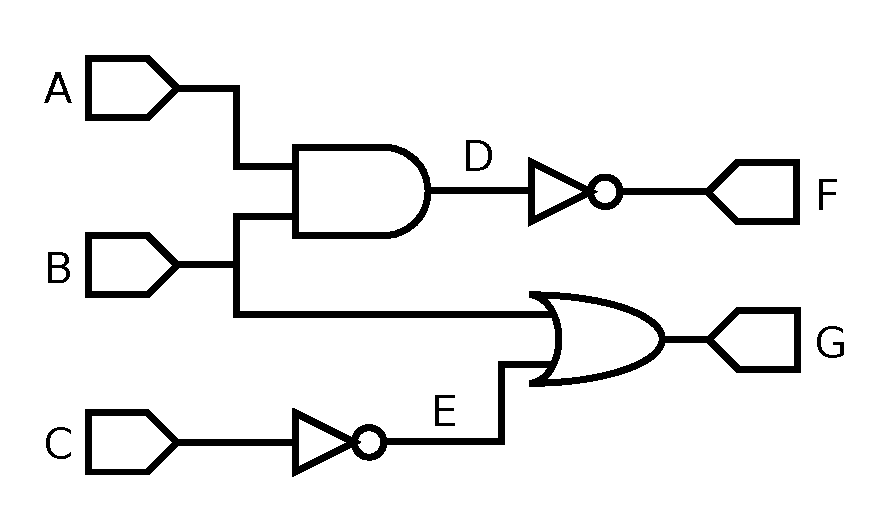
\includegraphics[width=0.75\textwidth]{example_fuzzy_logic_circuit}

The prior probability distributions that describe the input variables are given below:

\begin{tabular}{|c||c|c|c|}
\hline
\(A\) & \(0\) & \(1\) & \(2\) \\ 
\hline
\hline
\(\Pr(A)\) & 0.33 & 0.33 & 0.34 \\
\hline
\end{tabular}
~
\begin{tabular}{|c||c|c|c|}
\hline
\(B\) & \(0\) & \(1\) & \(2\) \\ 
\hline
\hline
\(\Pr(B)\) & 0.7 & 0.2 & 0.1 \\
\hline
\end{tabular}
~
\begin{tabular}{|c||c|c|c|}
\hline
\(C\) & \(0\) & \(1\) & \(2\) \\ 
\hline
\hline
\(\Pr(C)\) & 0.1 & 0.8 & 0.1 \\
\hline
\end{tabular}

\vspace{5mm}

\(D = A \;\text{AND}\; B\): A multivalued AND ideally returns the smaller of the two operands, but in this scenario, the output might not be pulled down to the smaller value. 

\(E = \text{NOT}\; C\): A multivalued NOT ideally returns the complement of the operand, but in this scenario, the output might not be pulled to the correct output.  

\begin{tabular}{|c||c|c|c|}
\hline
\(D\) & \(0\) & \(1\) & \(2\) \\ 
\hline
\hline
\(\Pr(D|A=0,B=0)\) & 1.00 & 0.00 & 0.00 \\
\hline
\(\Pr(D|A=0,B=1)\) & 0.90 & 0.10 & 0.00 \\
\hline
\(\Pr(D|A=0,B=2)\) & 0.80 & 0.10 & 0.10 \\
\hline
\(\Pr(D|A=1,B=0)\) & 0.90 & 0.10 & 0.00 \\
\hline
\(\Pr(D|A=1,B=1)\) & 0.00 & 1.00 & 0.00 \\
\hline
\(\Pr(D|A=1,B=2)\) & 0.00 & 0.90 & 0.10 \\
\hline
\(\Pr(D|A=2,B=0)\) & 0.80 & 0.10 & 0.10 \\
\hline
\(\Pr(D|A=2,B=1)\) & 0.00 & 0.90 & 0.10 \\
\hline
\(\Pr(D|A=2,B=2)\) & 0.00 & 0.00 & 1.00 \\
\hline
\end{tabular}
~
\begin{tabular}{|c||c|c|c|}
\hline
\(E\) & \(0\) & \(1\) & \(2\) \\
\hline
\hline
\(\Pr(E|C=0)\) & 0.10 & 0.10 & 0.80 \\ 
\hline
\(\Pr(E|C=1)\) & 0.10 & 0.80 & 0.10 \\ 
\hline
\(\Pr(E|C=2)\) & 0.80 & 0.10 & 0.10 \\ 
\hline
\end{tabular}

\vspace{5mm}

\(F = \text{NOT}\; D\): A multivalued NOT ideally returns the complement of the operand, but in this scenario, the output might not be pulled to the correct output.  

\(G = B \;\text{OR}\; E\): A multivalued OR ideally returns the larger of the two operands, but in this scenario, the output might not be pulled up to the larger value.

\begin{tabular}{|c||c|c|c|}
\hline
\(F\) & \(0\) & \(1\) & \(2\) \\
\hline
\hline
\(\Pr(F|D=0)\) & 0.10 & 0.10 & 0.80 \\ 
\hline
\(\Pr(F|D=1)\) & 0.10 & 0.80 & 0.10 \\ 
\hline
\(\Pr(F|D=2)\) & 0.80 & 0.10 & 0.10 \\ 
\hline
\end{tabular}
~
\begin{tabular}{|c||c|c|c|}
\hline
\(G\) & \(0\) & \(1\) & \(2\) \\ 
\hline
\hline
\(\Pr(G|B=0,E=0)\) & 1.00 & 0.00 & 0.00 \\
\hline
\(\Pr(G|B=0,E=1)\) & 0.10 & 0.90 & 0.00 \\
\hline
\(\Pr(G|B=0,E=2)\) & 0.10 & 0.10 & 0.80 \\
\hline
\(\Pr(G|B=1,E=0)\) & 0.10 & 0.90 & 0.00 \\
\hline
\(\Pr(G|B=1,E=1)\) & 0.00 & 1.00 & 0.00 \\
\hline
\(\Pr(G|B=1,E=2)\) & 0.00 & 0.10 & 0.90 \\
\hline
\(\Pr(G|B=2,E=0)\) & 0.10 & 0.10 & 0.80 \\
\hline
\(\Pr(G|B=2,E=1)\) & 0.00 & 0.10 & 0.90 \\
\hline
\(\Pr(G|B=2,E=2)\) & 0.00 & 0.00 & 1.00 \\
\hline
\end{tabular}

\vspace{5mm}

\begin{minipage}{\textwidth}
The decision diagram and syntax for \(\Pr(A)\):

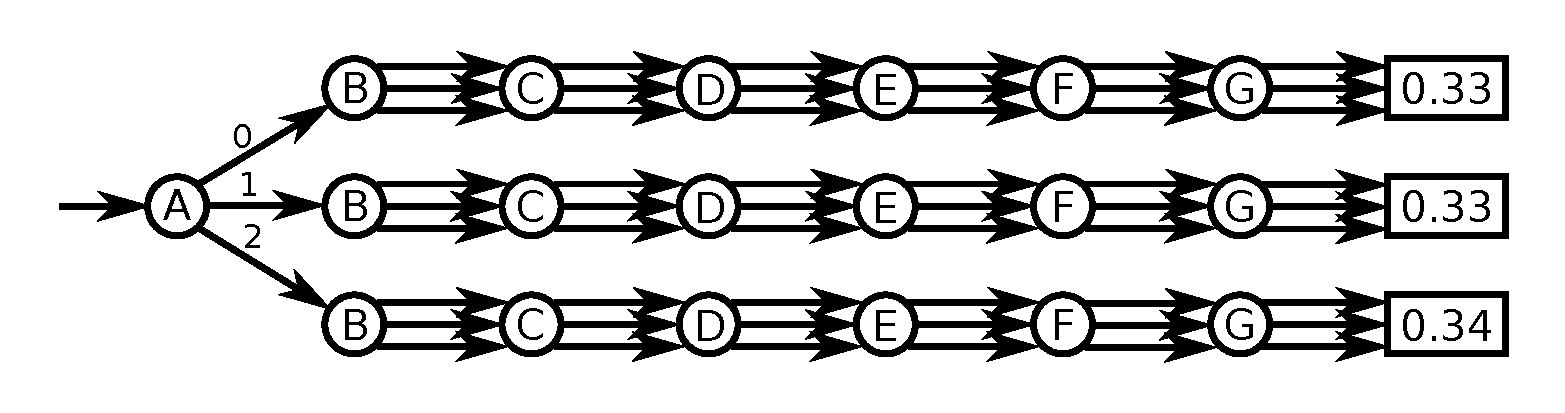
\includegraphics[width = \textwidth]{Pr(A)}

\begin{verbatim}
table 7 
normal   s "A" 3  inactive s "B" 3  inactive s "C" 3  inactive s "D" 3 
inactive s "E" 3  inactive s "F" 3  inactive s "G" 3 
0 
d 0.33  d 0.33  d 0.34 
\end{verbatim} 
\end{minipage}

\vspace{5mm}

\begin{minipage}{\textwidth}
The decision diagram and syntax for \(\Pr(B)\):

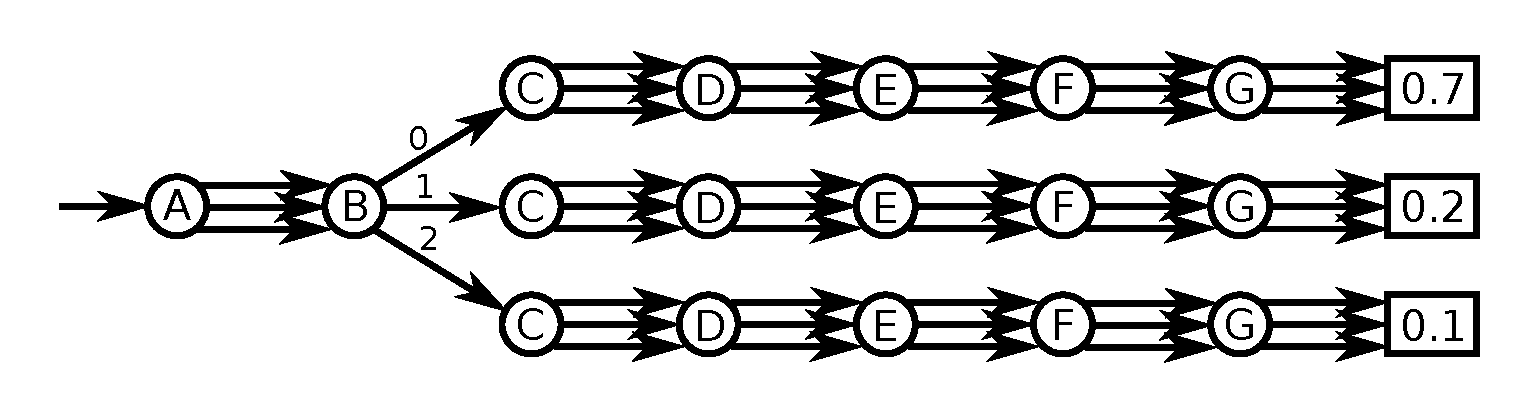
\includegraphics[width = \textwidth]{Pr(B)}

\begin{verbatim}
table 7
inactive s "A" 3  normal   s "B" 3  inactive s "C" 3  inactive s "D" 3 
inactive s "E" 3  inactive s "F" 3  inactive s "G" 3 
0 
d 0.7  d 0.2  d 0.1 
\end{verbatim}
\end{minipage}

\vspace{5mm}

\begin{minipage}{\textwidth}
The decision diagram and syntax for \(\Pr(C)\):

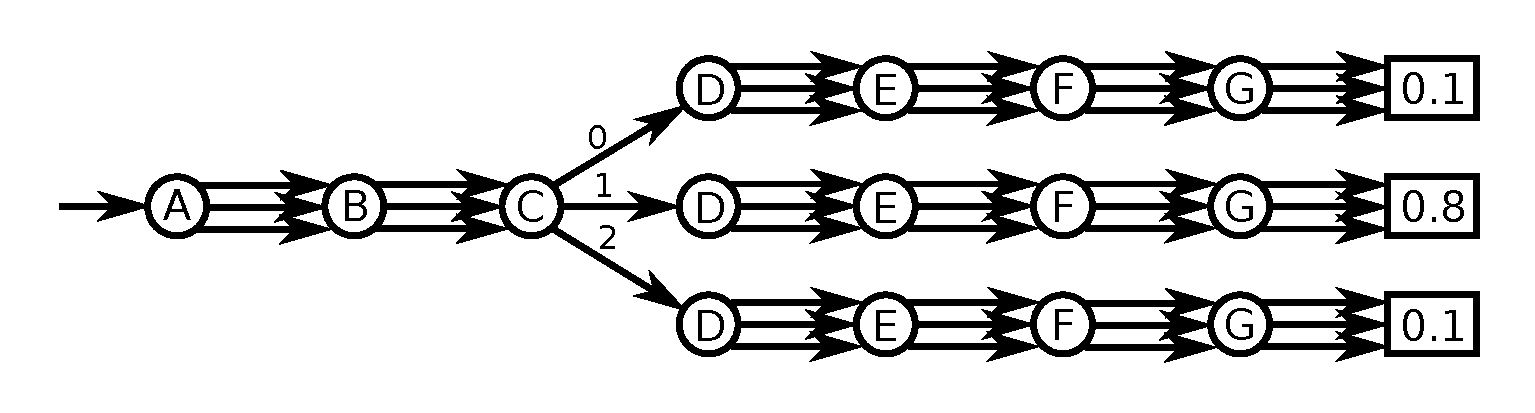
\includegraphics[width = \textwidth]{Pr(C)}

\begin{verbatim}
table 7
inactive s "A" 3  inactive s "B" 3  normal   s "C" 3  inactive s "D" 3 
inactive s "E" 3  inactive s "F" 3  inactive s "G" 3 
0 
d 0.1  d 0.8  d 0.1 
\end{verbatim}
\end{minipage}

\vspace{5mm}

\begin{minipage}{\textwidth}
The decision diagram and syntax for \(\Pr(D|A,B)\):

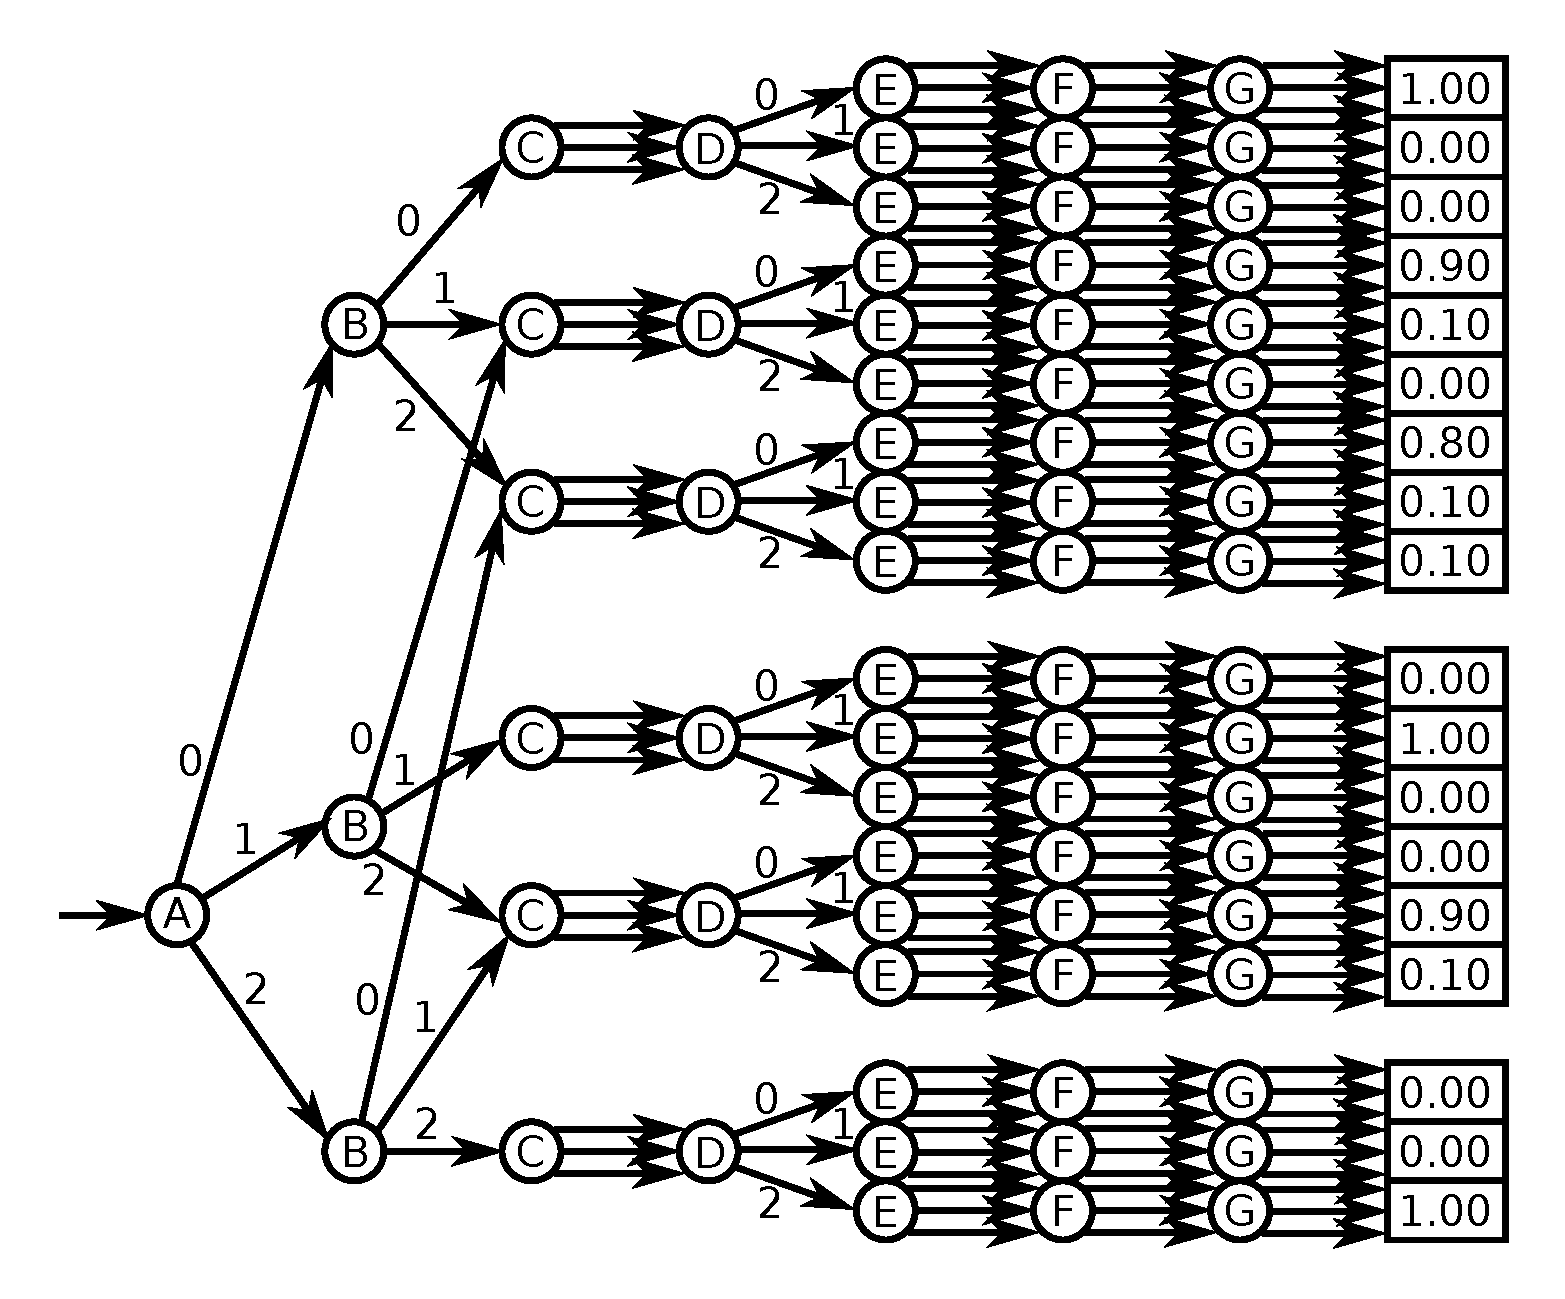
\includegraphics[width = \textwidth]{Pr(D)}
\end{minipage}

\begin{verbatim}
new s "A" < 
    {A=0} new s "B" < 
        {B=0} table 5
        inactive s "C" 3  normal   s "D" 3  inactive s "E" 3  inactive s "F" 3
        inactive s "G" 3 
        0 
        d 1.00  d 0.00  d 0.00 , 
        {B=1} table 5
        inactive s "C" 3  normal   s "D" 3  inactive s "E" 3  inactive s "F" 3
        inactive s "G" 3 
        0 
        d 0.90  d 0.10  d 0.00 , 
        {B=2} table 5
        inactive s "C" 3  normal   s "D" 3  inactive s "E" 3  inactive s "F" 3
        inactive s "G" 3 
        0 
        d 0.80  d 0.10  d 0.10 > , 
    {A=1} new s "B" <  
        {B=0} addr ! 0 1 @ , 
        {B=1} table 5
        inactive s "C" 3  normal   s "D" 3  inactive s "E" 3  inactive s "F" 3
        inactive s "G" 3 
        0 
        d 0.00  d 1.00  d 0.00 , 
        {B=2} table 5
        inactive s "C" 3  normal   s "D" 3  inactive s "E" 3  inactive s "F" 3
        inactive s "G" 3 
        0 
        d 0.00  d 0.90  d 0.10 > , 
    {A=2} new s "B" <  
        {B=0} addr ! 0 2 @ , 
        {B=1} addr ! 1 2 @ , 
        {B=2} table 5
        inactive s "C" 3  normal   s "D" 3  inactive s "E" 3  inactive s "F" 3
        inactive s "G" 3 
        0 
        d 0.00  d 0.00  d 1.00 > > 
\end{verbatim}

\vspace{5mm}

\begin{minipage}{\textwidth}
The decision diagram and syntax for \(\Pr(E|C)\):

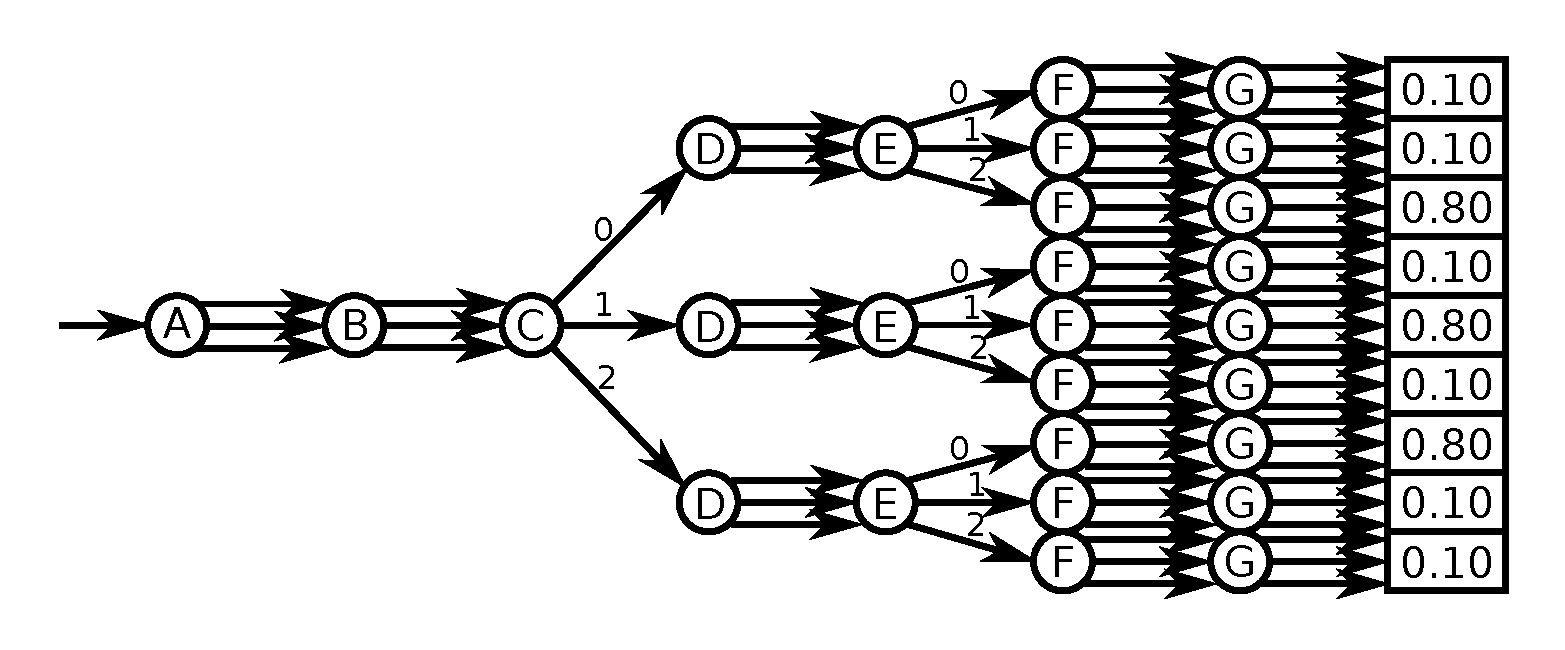
\includegraphics[width = \textwidth]{Pr(E)}

\begin{verbatim}
table 7 
inactive s "A" 3  inactive s "B" 3  normal   s "C" 3  inactive s "D" 3 
normal   s "E" 3  inactive s "F" 3  inactive s "G" 3 
0 
d 0.10  d 0.10  d 0.80   d 0.10  d 0.80  d 0.10   d 0.10  d 0.10  d 0.80 
\end{verbatim}
\end{minipage}

\vspace{5mm}

\begin{minipage}{\textwidth}
The decision diagram and syntax for \(\Pr(F|D)\):

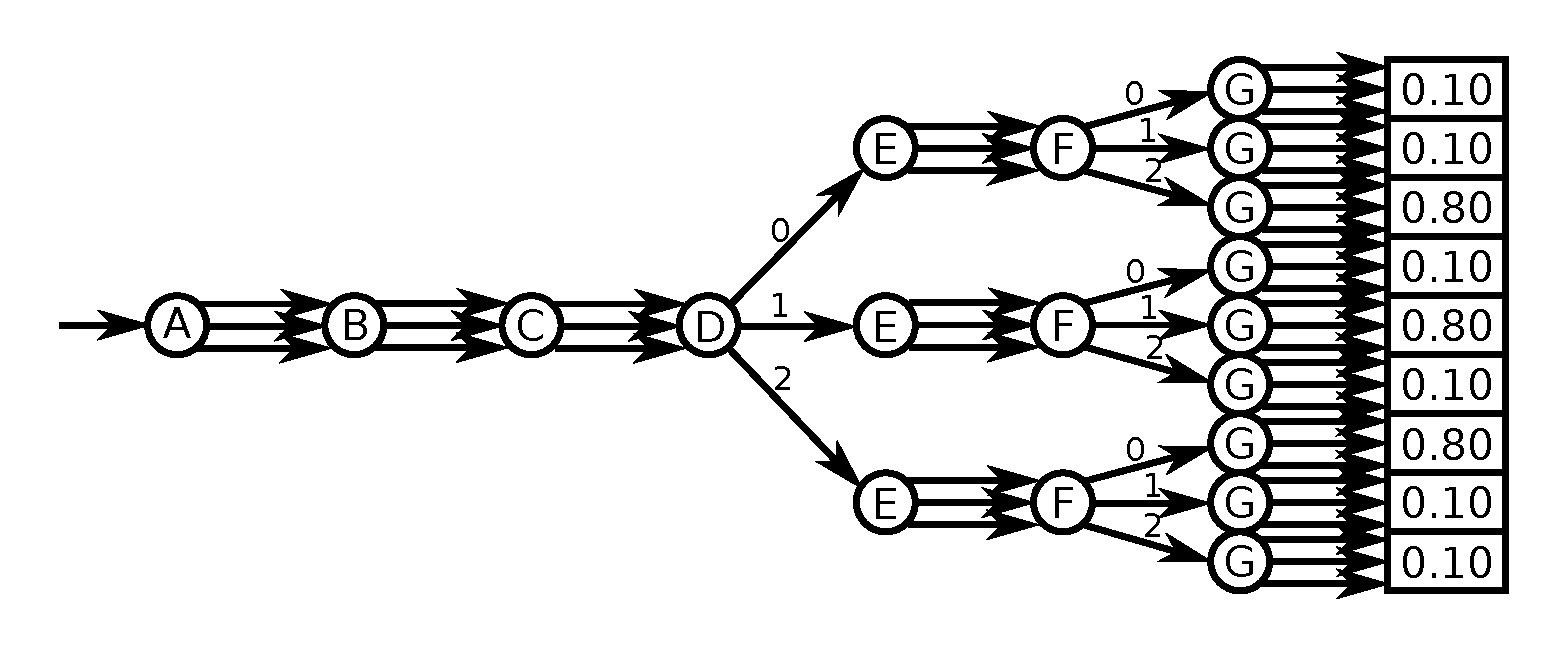
\includegraphics[width = \textwidth]{Pr(F)}

\begin{verbatim}
table 7 
inactive s "A" 3  inactive s "B" 3  inactive s "C" 3  normal   s "D" 3 
inactive s "E" 3  normal   s "F" 3  inactive s "G" 3 
0 
d 0.10  d 0.10  d 0.80   d 0.10  d 0.80  d 0.10   d 0.10  d 0.10  d 0.80 
\end{verbatim}
\end{minipage}

\vspace{5mm}

\begin{minipage}{\textwidth}
The decision diagram and syntax for \(\Pr(G|B,E)\):

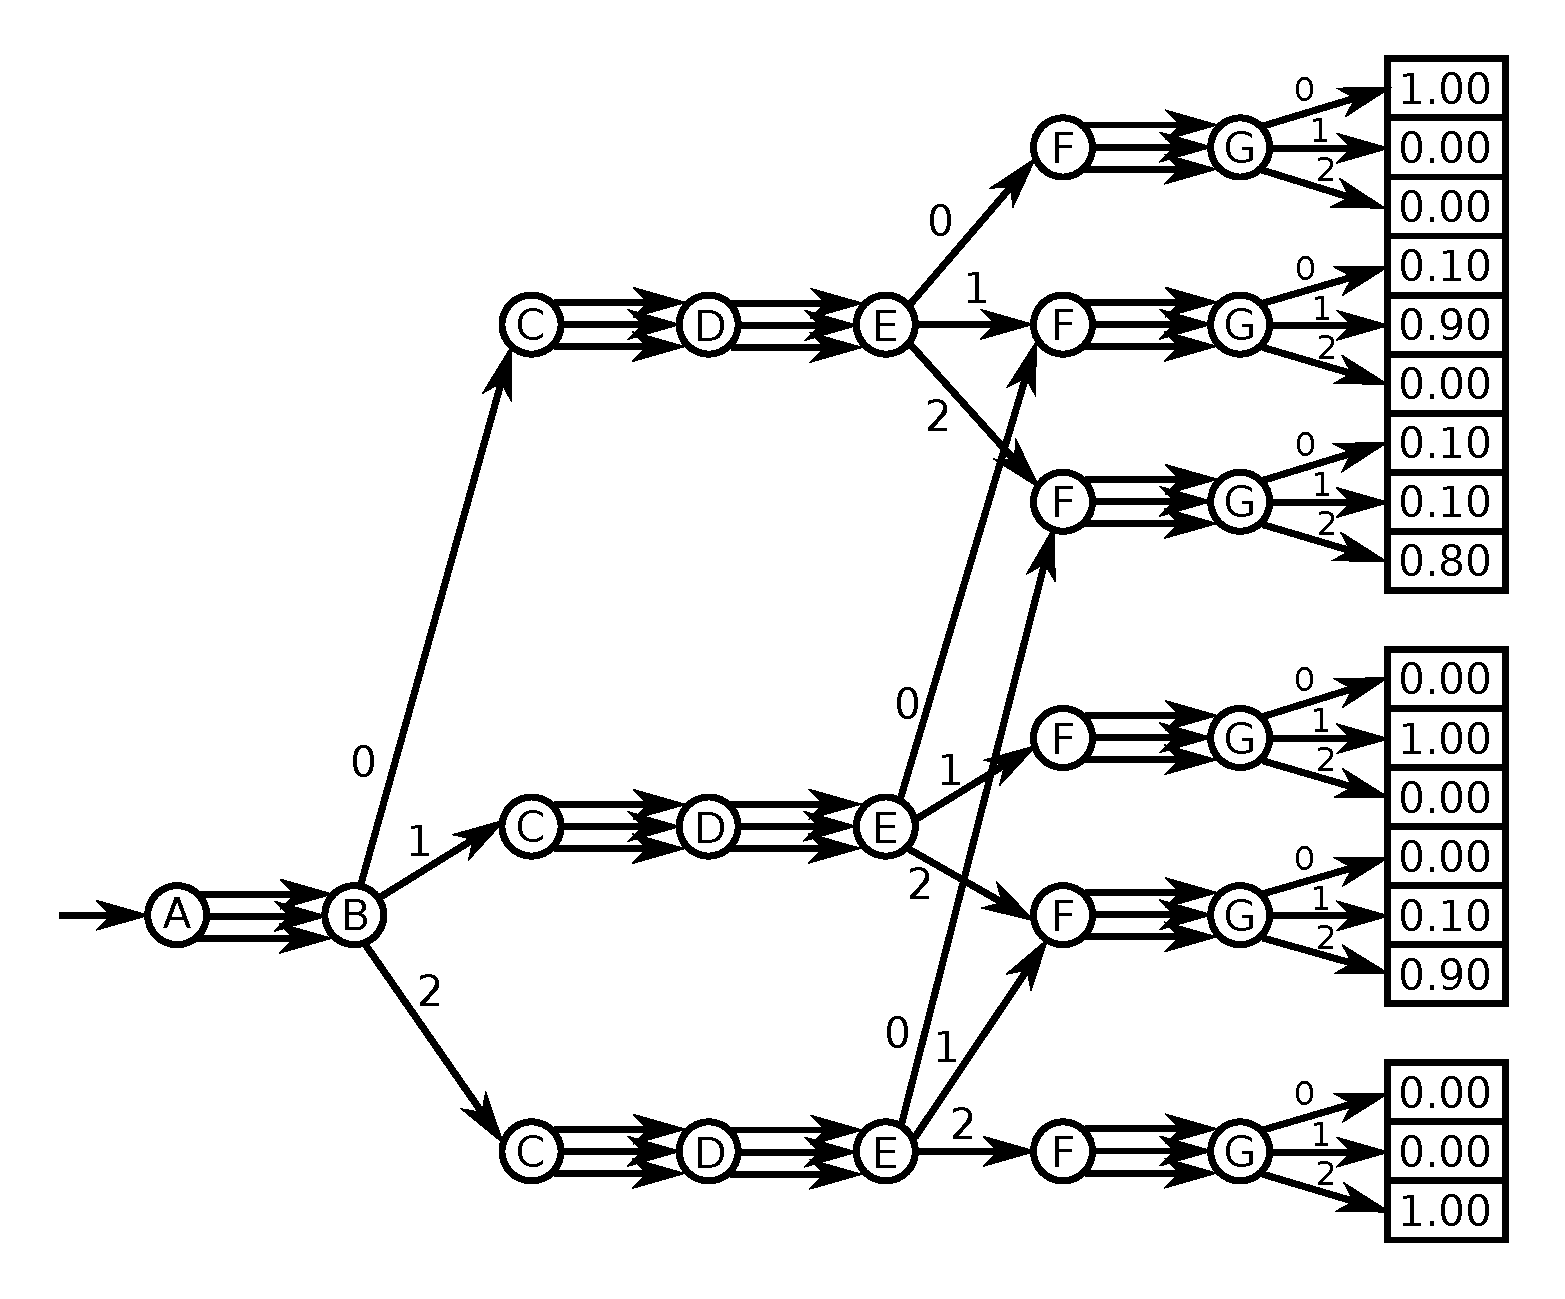
\includegraphics[width = \textwidth]{Pr(G)}
\end{minipage}

\begin{verbatim}
new s "A" < new s "B" < 
    {B=0} new s "C" < new s "D" < new s "E" < 
        {E=0} table 2
        inactive s "F" 3  normal   s "G" 3 
        0
        d 1.00  d 0.00  d 0.00 , 
        {E=1} table 2
        inactive s "F" 3  normal   s "G" 3 
        0
        d 0.10  d 0.90  d 0.00 , 
        {E=2} table 2
        inactive s "F" 3  normal   s "G" 3 
        0
        d 0.10  d 0.10  d 0.80 > , 
    addr 0 @ , addr 0 @ > , addr 0 @ , addr 0 @ > , 
    {B=1} new s "C" < new s "D" < new s "E" < 
        {E=0} addr ! 0 0 0 0 1 @ , 
        {E=1} table 2
        inactive s "F" 3  normal   s "G" 3 
        0
        d 0.00  d 1.00  d 0.00 , 
        {E=2} table 2
        inactive s "F" 3  normal   s "G" 3 
        0
        d 0.00  d 0.10  d 0.90 > , 
    addr 0 @ , addr 0 @ > , addr 0 @ , addr 0 @ > , 
    {B=2} new s "C" < new s "D" < new s "E" < 
        {E=0} addr ! 0 0 0 0 2 @ , 
        {E=1} addr ! 0 1 0 0 2 @ , 
        {E=2} table 2
        inactive s "F" 3 
        normal   s "G" 3 
        0
        d 0.00  d 0.00  d 1.00 > , 
    addr 0 @ , addr 0 @ > , addr 0 @ , addr 0 @ > > , 
addr 0 @ , addr 0 @ >        
\end{verbatim}

\subsection{Probabilistic Inference Example}

This section will detail using the above data alongside the above instructions to extract data about the above noisy ternary logic circuit. 

Consider a scenario where it is known that \(A = 1\), \(B=0\), and \(C=0\). Of interest is the joint marginal probability distribution for the outputs \(F\) and \(G\).   

The contents of the instructions file \texttt{Test Files/1\_instructions.txt} is:

\begin{verbatim}

{Applying the evidence}

copy_subgraph "Pr(A|evidence)" "Pr(A)"
condition "Pr(A|evidence)" 0 "Pr(A|evidence)" 0 1
condition "Pr(A|evidence)" 0 "Pr(A|evidence)" 1 0 
condition "Pr(A|evidence)" 0 "Pr(A|evidence)" 2 0 

copy_subgraph "Pr(B|evidence)" "Pr(B)"
condition "Pr(B|evidence)" 0 "Pr(B|evidence)" 0 1
condition "Pr(B|evidence)" 0 "Pr(B|evidence)" 1 0 
condition "Pr(B|evidence)" 0 "Pr(B|evidence)" 2 0 

copy_subgraph "Pr(C|evidence)" "Pr(C)"
condition "Pr(C|evidence)" 0 "Pr(C|evidence)" 0 1
condition "Pr(C|evidence)" 0 "Pr(C|evidence)" 1 0 
condition "Pr(C|evidence)" 0 "Pr(C|evidence)" 2 0 

copy_subgraph "Pr(D|evidence)" "Pr(D|A,B)"
condition "Pr(D|evidence)" 0 "Pr(D|evidence)" 0 1
condition "Pr(D|evidence)" 0 "Pr(D|evidence)" 1 0 
condition "Pr(D|evidence)" 0 "Pr(D|evidence)" 2 0

copy_subgraph "Pr(E|evidence)" "Pr(E|C)"
condition "Pr(E|evidence)" 0 "Pr(E|evidence)" 0 1
condition "Pr(E|evidence)" 0 "Pr(E|evidence)" 1 0 
condition "Pr(E|evidence)" 0 "Pr(E|evidence)" 2 0  

copy_subgraph "Pr(F|evidence)" "Pr(F|D)"
condition "Pr(F|evidence)" 0 "Pr(F|evidence)" 0 1
condition "Pr(F|evidence)" 0 "Pr(F|evidence)" 1 0 
condition "Pr(F|evidence)" 0 "Pr(F|evidence)" 2 0 

copy_subgraph "Pr(G|evidence)" "Pr(G|B,E)"
condition "Pr(G|evidence)" 0 "Pr(G|evidence)" 0 1
condition "Pr(G|evidence)" 0 "Pr(G|evidence)" 1 0 
condition "Pr(G|evidence)" 0 "Pr(G|evidence)" 2 0 

{multiplying together the conditioned factors}

binary_operator "Pr(total)" * 1 "Pr(A|evidence)" "Pr(B|evidence)"
binary_operator "Pr(total)" * 1 "Pr(total)" "Pr(C|evidence)"
binary_operator "Pr(total)" * 1 "Pr(total)" "Pr(D|evidence)"
binary_operator "Pr(total)" * 1 "Pr(total)" "Pr(E|evidence)"
binary_operator "Pr(total)" * 1 "Pr(total)" "Pr(F|evidence)"
binary_operator "Pr(total)" * 1 "Pr(total)" "Pr(G|evidence)"

{marginalizing out the unnecessary variables}

marginalize "Pr(total)" 0 "Pr(total)" 3
marginalize "Pr(total)" 0 "Pr(total)" 4

{calculating and applying the normalization constant}

copy_subgraph "Z" "Pr(total)" 
marginalize "Z" 1 "Z" 5 
marginalize "Z" 1 "Z" 6 

binary_operator "Pr(total)" / 1 "Pr(total)" "Z" 

{print the posterior probabilities}

assign_node "probe" "Pr(total)" 7 0 0 0 0 0 0 0 
print_data "probe"
assign_node "probe" "Pr(total)" 7 0 0 0 0 0 0 1 
print_data "probe"
assign_node "probe" "Pr(total)" 7 0 0 0 0 0 0 2 
print_data "probe"
print_string ""
assign_node "probe" "Pr(total)" 7 0 0 0 0 0 1 0 
print_data "probe"
assign_node "probe" "Pr(total)" 7 0 0 0 0 0 1 1 
print_data "probe"
assign_node "probe" "Pr(total)" 7 0 0 0 0 0 1 2 
print_data "probe"
print_string ""
assign_node "probe" "Pr(total)" 7 0 0 0 0 0 2 0 
print_data "probe"
assign_node "probe" "Pr(total)" 7 0 0 0 0 0 2 1 
print_data "probe"
assign_node "probe" "Pr(total)" 7 0 0 0 0 0 2 2 
print_data "probe"

\end{verbatim}

The contents of \texttt{Test Files/1\_output.txt} is:

\begin{verbatim}
d 0.019000

d 0.017000

d 0.064000



d 0.032300

d 0.028900

d 0.108800



d 0.138700

d 0.124100

d 0.467200
\end{verbatim}

This yields the following posterior probability distribution over \(F\) and \(G\):

\begin{tabular}{|c||c|c|c|}
\hline
\(G\) & 0 & 1 & 2 \\
\hline
\hline
\(\Pr(F=0,G)\) & 0.0190 & 0.0170 & 0.0640 \\ 
\(\Pr(F=1,G)\) & 0.0323 & 0.0289 & 0.1088 \\
\(\Pr(F=2,G)\) & 0.1387 & 0.1241 & 0.4672 \\
\hline
\end{tabular}

\end{document}









